% !TEX root = ../main.tex
\subsection{FMT Efficiency}
    % Low FMT efficiency + list sources.
    Compared to the alignment work described in section \ref{sec::fmt_alignment_and_reconstruction}, a low FMT is observed in this analysis.
    This can be seen in figure \ref{fig::vz_012933}.
    Upon inspection, three causes can be blamed for this: the application of incorrect alignment constants, a geometry effect, and a general FMT offline reconstruction issue.

    \begin{figure}[b!]
        \centering\frame{
        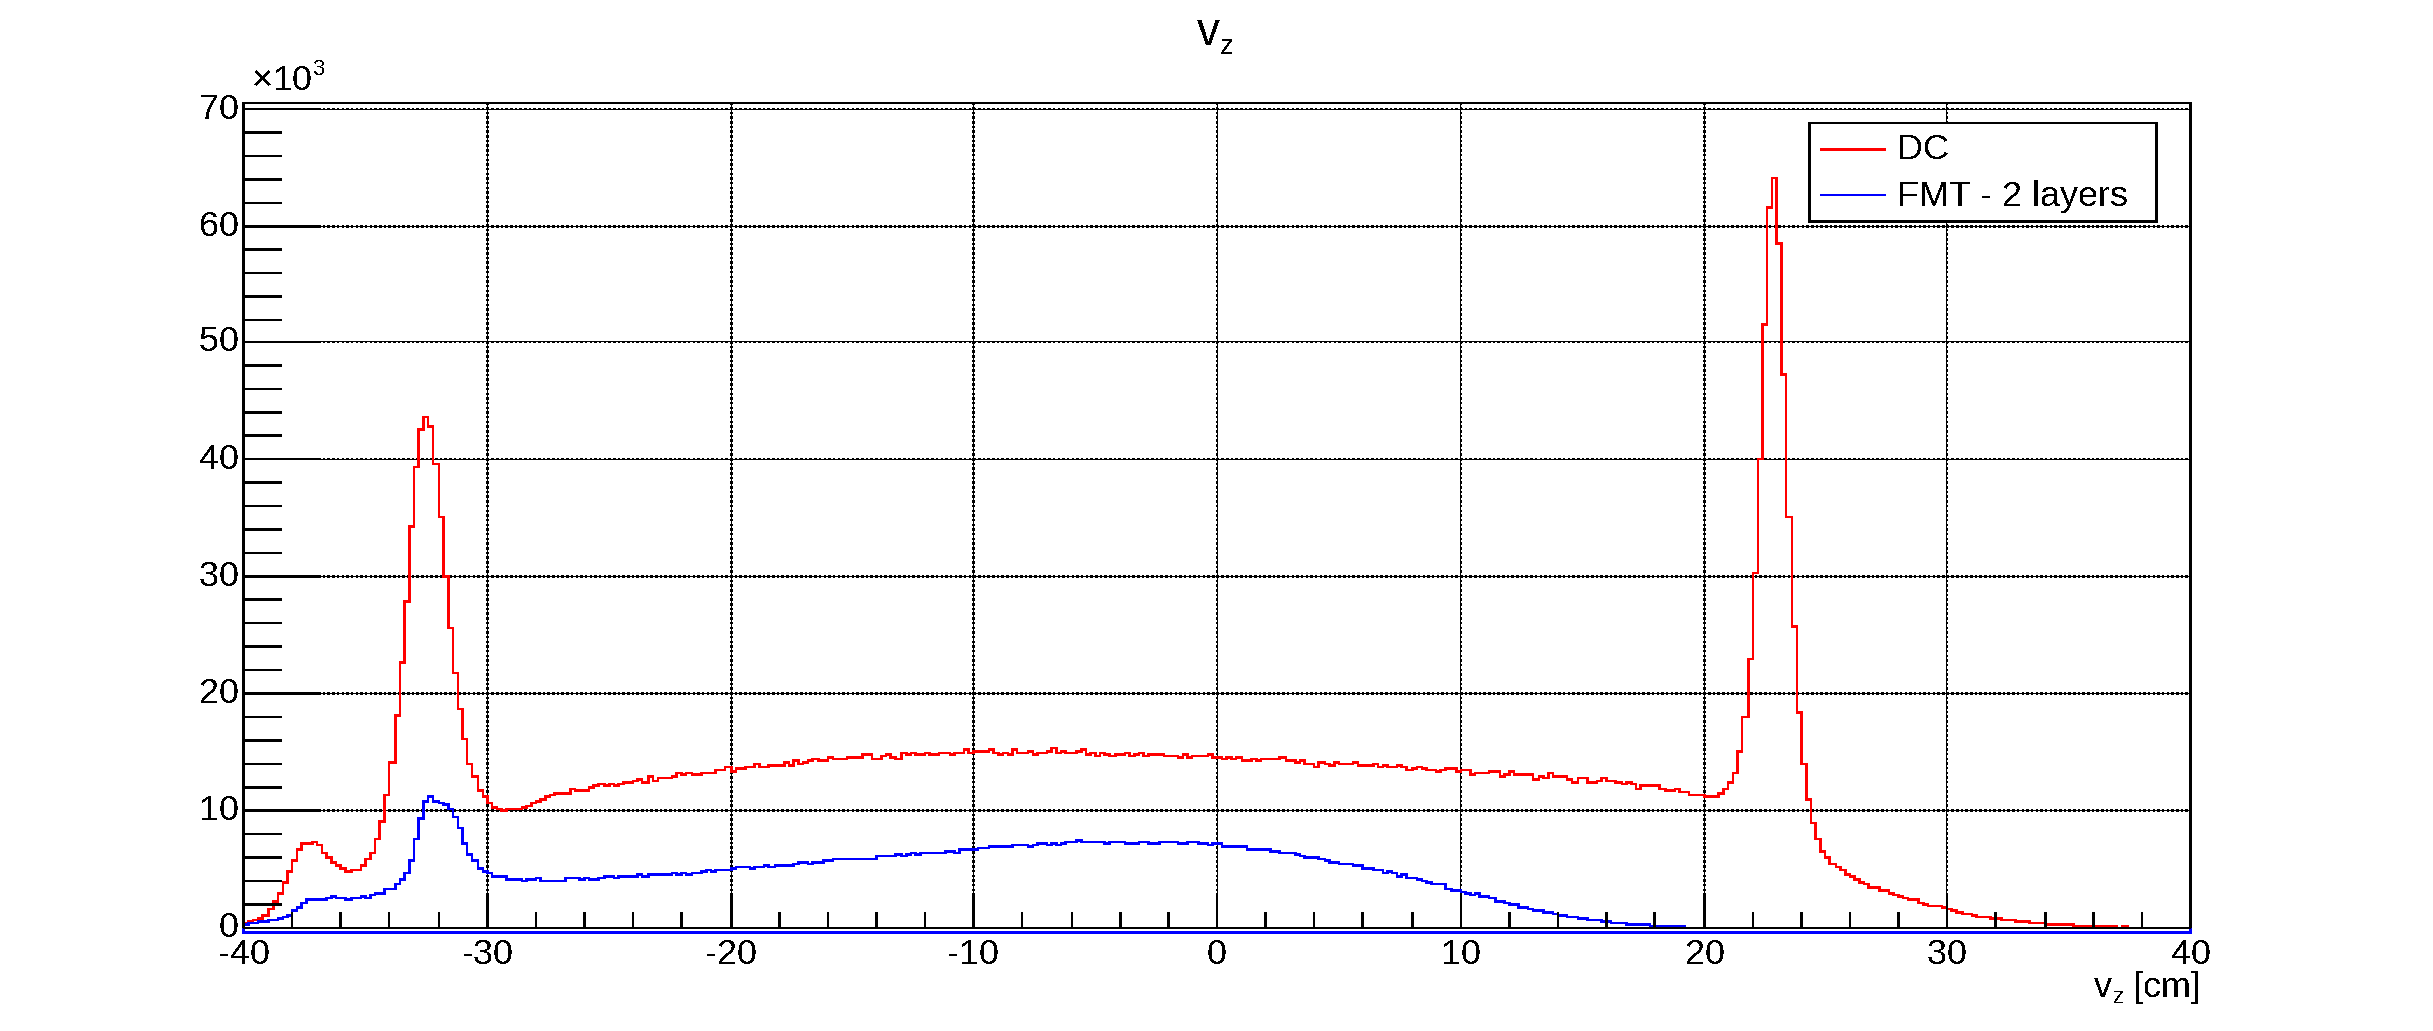
\includegraphics[width=\textwidth]{14resultsandconclusions/img/10vz_012933.pdf}}
        \caption[$v_z$ for DC and FMT, run 12933]{$v_z$ for DC (in red) and FMT (in blue). Summer 2020 data, run 12933. The wide peaks in FMT suggest an uncorrected misalignment.}
        \label{fig::vz_012933}
    \end{figure}

    % !TEX root = ../main.tex
\subsubsection{Alignment Effect}
    % Introduction: The problem.
    The RG-F experiment's data is divided based on the season over which runs take place, thus there is Spring 2020 and Summer 2020 data.
    Based on the run group's guidelines, it is recommended to use Summer data, as it has seen more calibration than the Spring data.
    However, this calibration work hasn't included the FMT detector, and a strong misalignment effect is observed.

    % Cause of the problem.
    By simple visual inspection, two peaks can be clearly seen between $z = -36$ cm and $z = -30$ cm in figure \ref{fig::dc_vs_fmt_vz_011983}.
    These peaks are merged in figure \ref{fig::vz_012933}.
    As discussed in section \ref{sec::fmtalignmentandreconstruction}, this issue comes from a lack of correction for FMT misalignments.

    % Solution.
    The simplest solution is to use Spring data.
    While more work has been put on Summer data, it mainly pertains to the central detector; unrelated to this analysis.
    Figure \ref{fig::vz_012016} shows the same $v_z$ plot from Spring 2020 run 12016.
    Both peaks are clearly visible in this plot, suggesting that misalignments are properly accounted for in the run.

    \begin{figure}[t!]
        \centering\frame{
        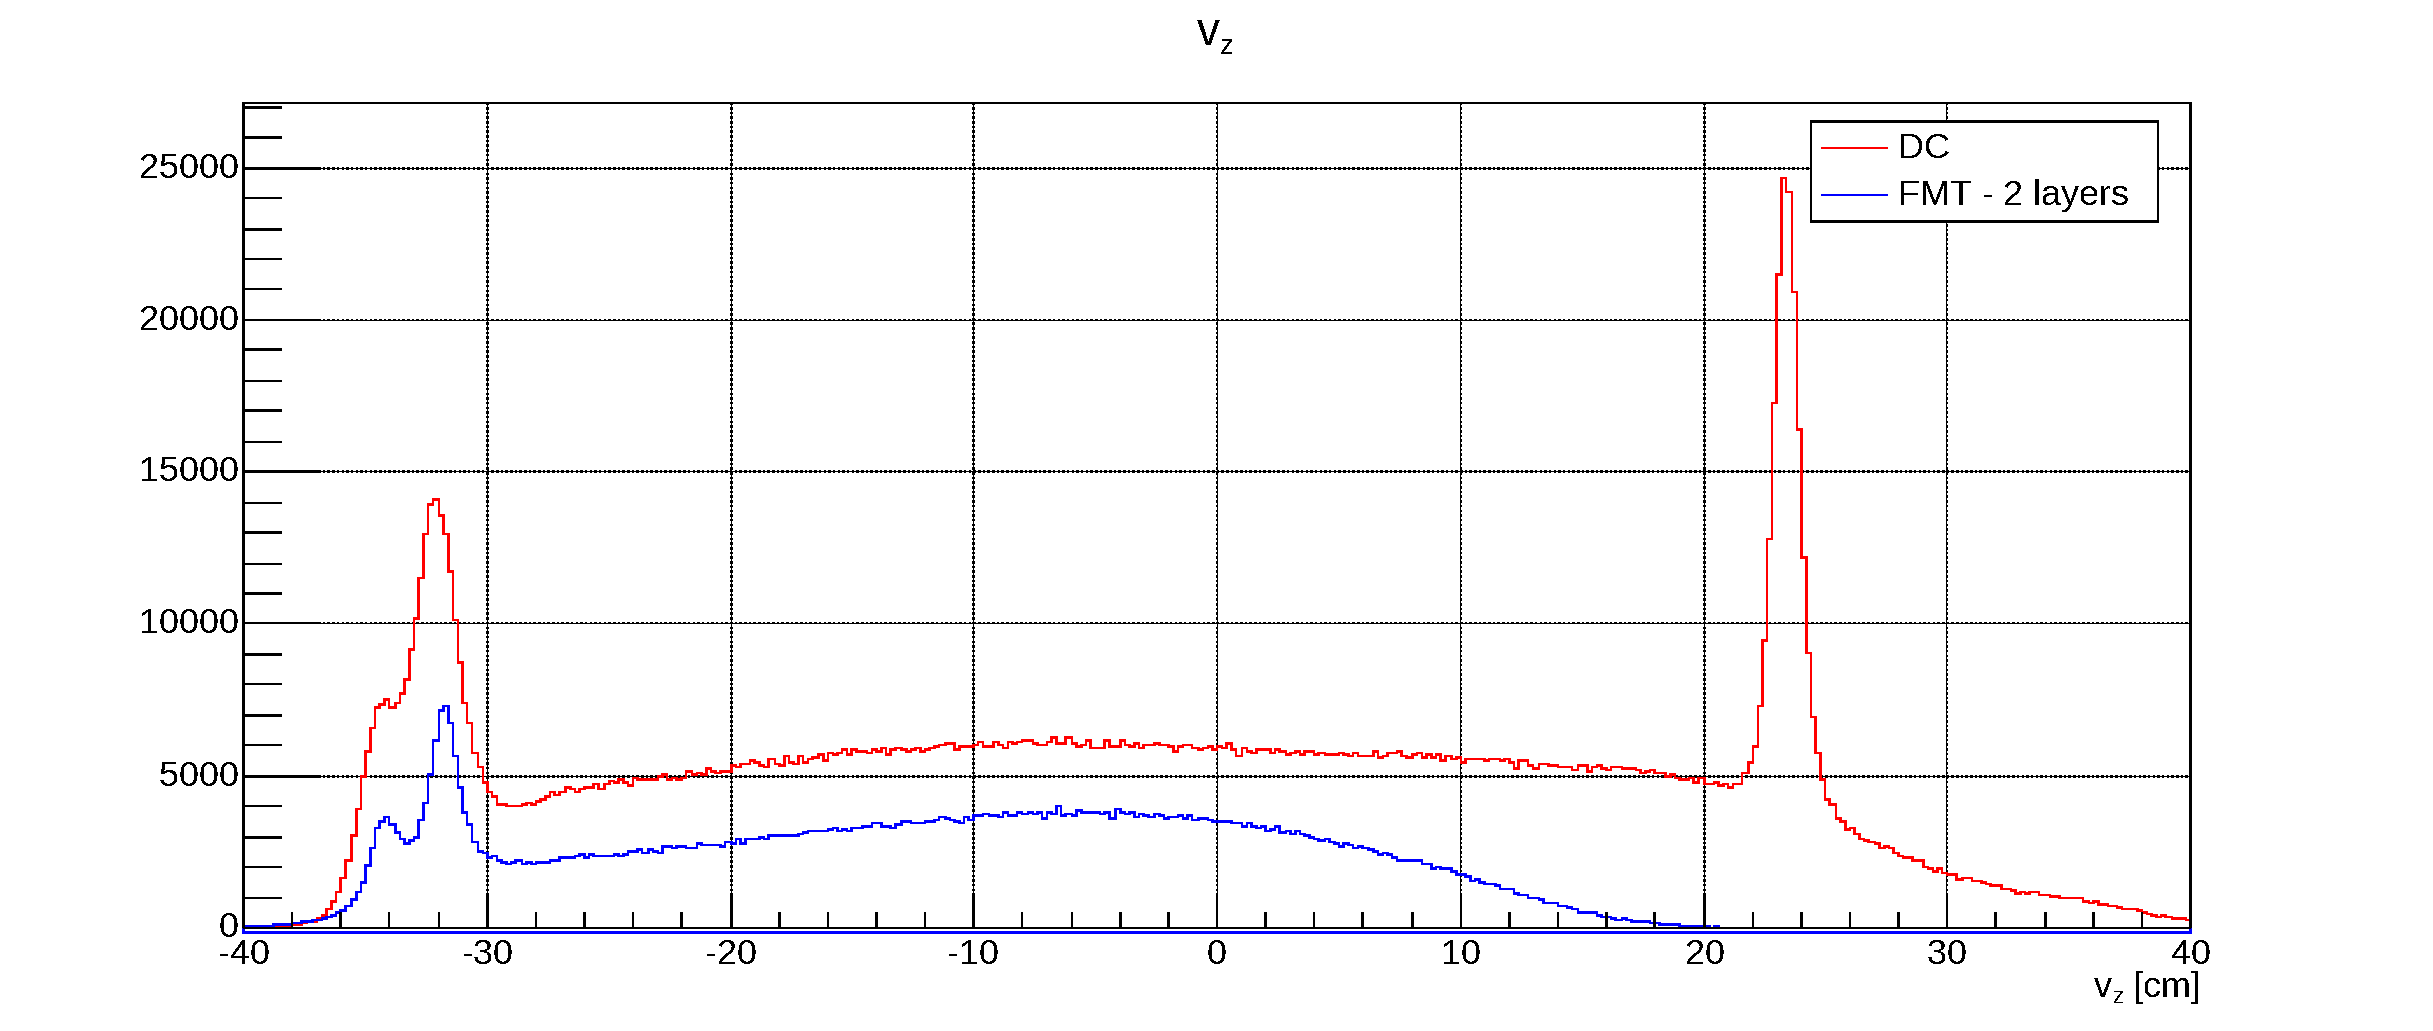
\includegraphics[width=\textwidth]{14resultsandconclusions/img/11vz_012016.pdf}}
        \caption[$v_z$ for DC and FMT, run 12016]{$v_z$ for DC (in red) and FMT (in blue). Spring 2020 data, run 12016. The upstream twin peaks can be clearly distinguished, suggesting a correct misalignment correction.}
        \label{fig::vz_012016}
    \end{figure}

    % !TEX root = ../main.tex
\subsubsection{Geometry Effect}
    % The effect has already been presented and discussed before, so we're brief.
    This problem is already discussed in detail in section \ref{ssec::validationandresults}.
    As a quick reminder, FMT sits at $z \approx 26$ cm, and it naturally performs poorly for targets to close to it.
    We can measure the strength of this effect by applying the geometry cut given by equation \eqref{eq::fmt_geometry_cut} to both DC and FMT tracks.
    Figure \ref{fig::vz_012016_geomcut} the effect of the cut when applied on figure \ref{fig::vz_012016}.
    Its effect on a $v_z$ vs $\theta$ plot can be seen on figure \ref{fig::vz_vs_theta}.

    Based on this cut and the FMT $z$ position, subsequent plots will be constrained to the range $-30 \text{[cm]} < v_z < 20 \text{[cm]}$.

    \begin{figure}[h!]
        \centering\frame{
        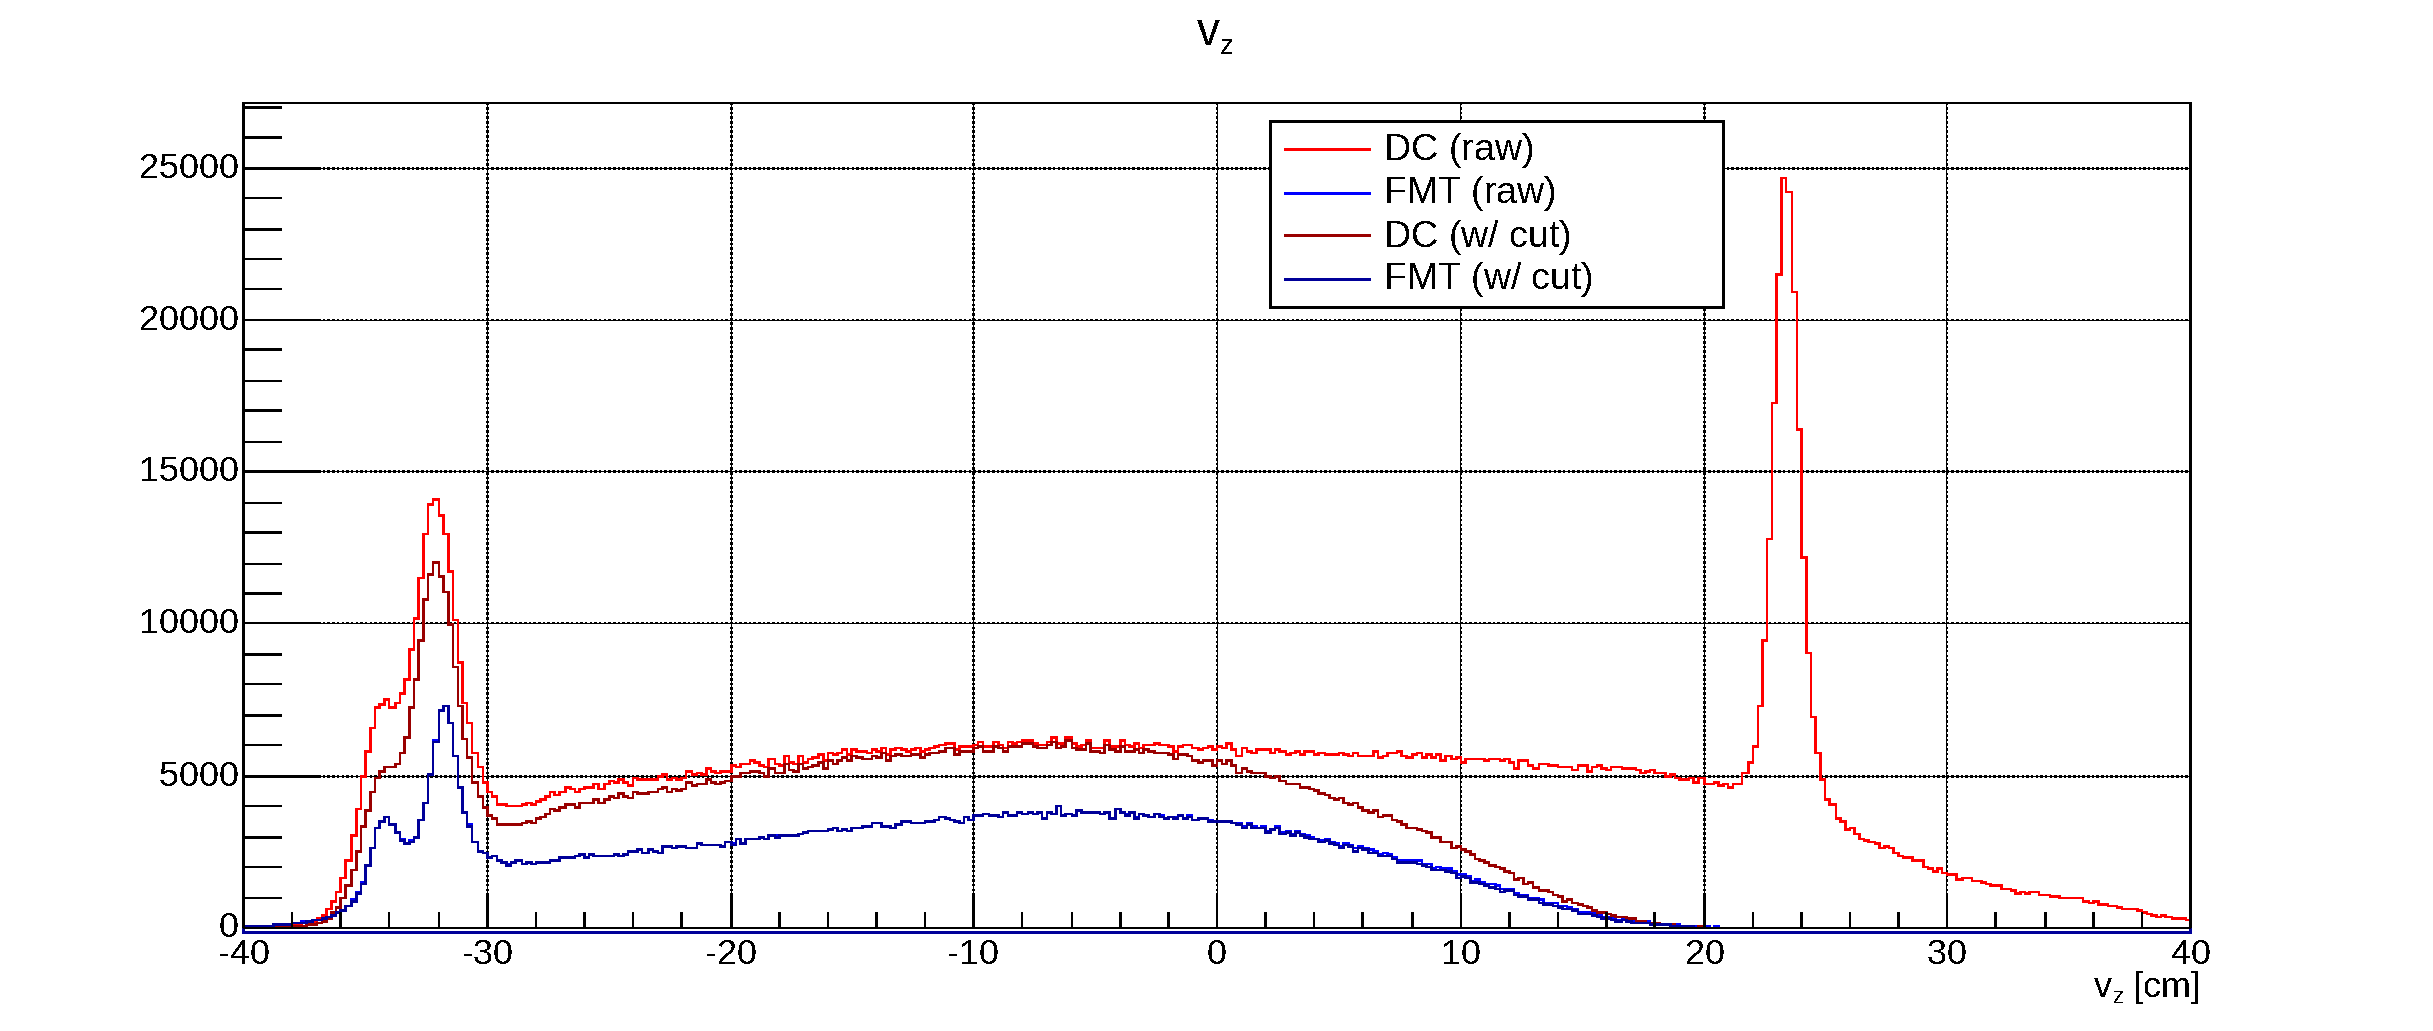
\includegraphics[width=\textwidth]{14resultsandconclusions/img/12vz_012016_geomcut.pdf}}
        \caption[$v_z$ for DC and FMT, w/ and w/out the geometry cut, run 12016]{$v_z$ for DC without the geometry cut (in red), with it (in dark red), for FMT without it (in blue), and with it (in dark blue). Spring 2020 data, run 12016. The effect is very clear on DC tracks, yet it almost doesn't affect FMT tracks.}
        \label{fig::vz_012016_geomcut}
    \end{figure}

    % !TEX root = ../main.tex
\subsubsection{Reconstruction Effect}
    Even after correcting for both the alignment and geometry issues, FMT still has a lower efficiency when compared to that found during alignment (compare figures \ref{fig::vz_012016_geomcut} with \ref{fig::dc_vs_fmt_vz_011983_corrected}).
    After some study, the effect was found not to be correlated to run number, beam energy, or beam luminosity.
    Based on this, we can discard it being caused by hardware issues or run conditions.

    Based on this, the logical conclusion is that the effect comes from a general issue in FMT offline reconstruction.
    Finding and fixing this would be a larger project than what's contemplated in the scope of this thesis, so it's left as future work.
    For the purposes of this analysis, we'll contempt ourselves with using a large number of events, minimising statistic deficiencies.

    % !TEX root = ../main.tex
\subsubsection{Efficiency Study}
% --+ Integrated. +---------------------------------------------------------
    With all these effects accounted for, we can proceed to study the efficiency in detail.
    First, if we define FMT efficiency as the percentage of DC tracks that get accepted by FMT, we get table \ref{tab::fmt_efficiency_study} for runs 12933 (Summer 2020) and 12016 (Spring 2020).

    \begin{center}
        \begin{tabularx}{0.70\textwidth}{Xr|rrcrr}
            & & \multicolumn{2}{l}{\textbf{Run 12933}}        & & \multicolumn{2}{l}{\textbf{Run 12016}} \\
                                   &          & raw  & w/ cut & & raw  & w/ cut \\
            \hline
            \textbf{Triggers}      & 2 layers & 25\% & 37\%   & & 33\% & 54\%   \\
                                   & 3 layers &  5\% &  8\%   & & 10\% & 16\%   \\
            \hline
            \textbf{All particles} & 2 layers & 14\% & 27\%   & & 19\% & 43\%   \\
                                   & 3 layers &  2\% &  5\%   & &  5\% & 11\%
        \end{tabularx}
        \label{tab::fmt_efficiency_study}
    \end{center}

    By switching from Summer to Spring data, we see a $\sim32\%$ increase in trigger electrons detected, and a $\sim36\%$ in all particles.
    Then, by applying the geometry cut in $v_z$ and $\theta$, $\sim64\%$ more trigger electrons are detected (for a $\sim184\%$ total increase), and $\sim126\%$ more particles in general are detected (for a $\sim207\%$ total increase).

% --+ Separated. +----------------------------------------------------------
    We can then check how the efficiency changes as result of the corrections.
    Due to the geometric cut, we expect a strong dependency on $v_z$ and $\theta$, and at most a weak one on $\phi$ and $p$.
    This is what we see in data, as is shown in figure \ref{fig::fmt_efficiencies}.

    \begin{figure}[t!]
        \centering\frame{
        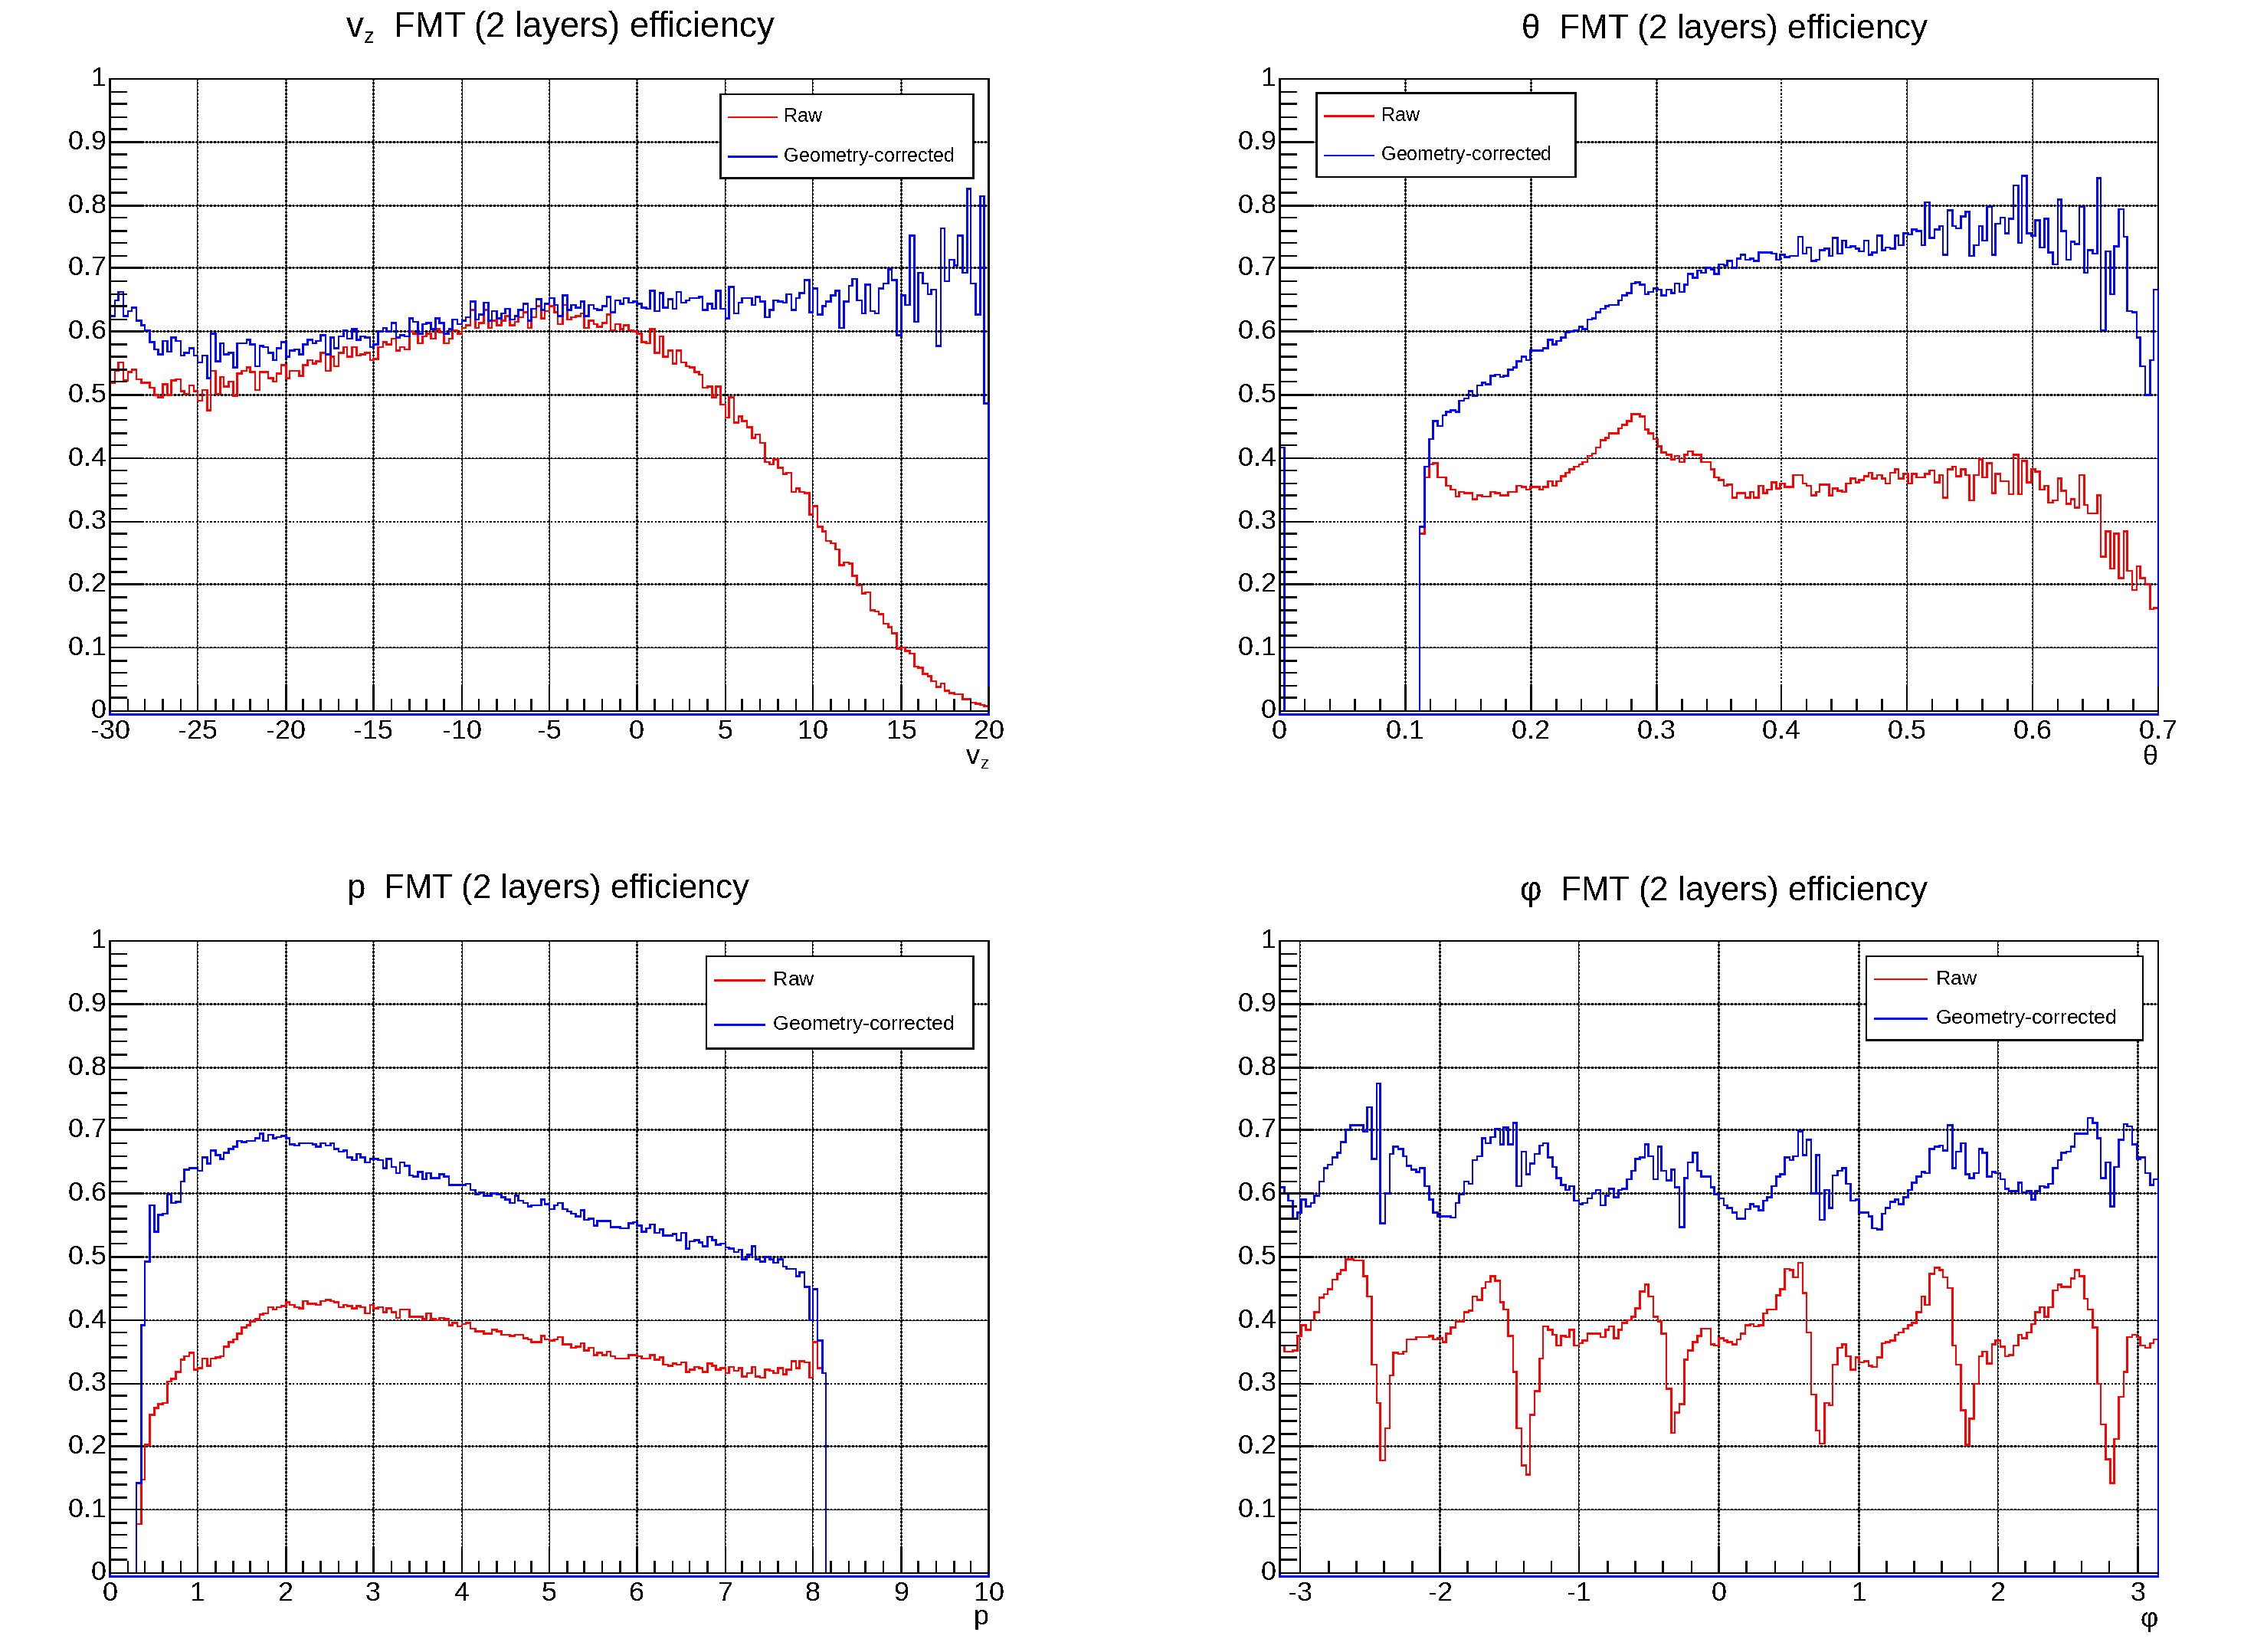
\includegraphics[width=\textwidth]{14resultsandconclusions/img/14efficiencies.pdf}}
        \caption[$v_z$, $\theta$, $\phi$, and $p$ efficiencies for FMT tracks, run 12016]{$v_z$, $\theta$, $\phi$, and $p$ efficiencies for FMT tracks. FMT Efficiency is defined as the percentage of DC tracks that are detected by 2 FMT layers. Run 12016.}
        \label{fig::fmt_efficiencies}
    \end{figure}

